%%%%%%%%%%%%%%%%%%%%%%%%%%%%%%%%%%%%%%%%%%%%%%%%%%%%%%%
% A template for Wiley article submissions to Networks.
% Developed by Overleaf.
%
% Modified by D. Shier  (13 Feb 2019)
%%
% Usage notes:
% % Use "num-refs" option for numerical citation and references style.
% % Use the attached wiley-networks.cls and abbrv_networks.bst files.

\documentclass[num-refs]{wiley-networks}

% Add additional packages here if required


% Update article type if known
\papertype{Original Article}
\paperfield{Networks} 

\title{This is my title}

% Use the \authfn to add symbols for additional footnotes and present addresses, if any. Usually start with 1 for notes about author contributions; then continuing with 2 etc if any author has a different present address.

\author[1\authfn{1}]{Author One}
\author[2\authfn{1}]{Author A.~Two}
\author[2\authfn{2}]{Author Three}
\author[2]{Author B.~Four}

\contrib[\authfn{1}]{Equally contributing authors.}


% Include full affiliation details for all authors
\affil[1]{Department, Institution, City, State or Province, Postal Code, Country}
\affil[2]{Department, Institution, City, State or Province, Postal Code, Country}

\corraddress{Author One, Department, Institution, City, State or Province, Postal Code, Country}
\corremail{correspondingauthor@email.com}

\presentadd[\authfn{2}]{Department, Institution, City, State or Province, Postal Code, Country}

\fundinginfo{Funder One, Funder One Department, Grant/Award Numbers: 123456 and 123458; Funder Two, Funder Two Department, Grant/Award Number: 123459}

% Include the name of the author that should appear in the running header
\runningauthor{Author One et al.}


\begin{document}

\maketitle

\begin{abstract}
This article studies the problem of transport of discrete items through multiple transportation modes, such as air freight, truck, and drone delivery systems. We establish theoretical bounds on the mean elapsed shipment time as well as the associate standard deviations. Empirical studies complement this contribution and show the effectiveness of the developed heuristic in closely approximating the true parameter values.


% Please include a minimum of six keywords
\keywords{keyword 1, keyword 2, keyword 3, keyword 4, keyword 5, keyword 6, keyword 7}
\end{abstract}

\section{First Level Heading}
Please lay out your article using the section headings and example objects below, and remember to delete all help text prior to submitting your article to the journal.



\subsection{Second Level Heading}
If data, scripts, or other artifacts used to generate the analyses presented in the article are available via a publicly available data repository, please include a reference to the location of the material within the article.

% Equations should be inserted using standard LaTeX equation and eqnarray environments, not as graphics, and should be set in the main text
This is an equation, numbered
\begin{equation}
\int_0^{+\infty}e^{-x^2}dx=\frac{\sqrt{\pi}}{2},
\end{equation}
as well as on one that is not numbered
\begin{equation*}
e^{i\pi}=-1
\end{equation*}

We can also have multiline expressions, as shown next:
\begin{eqnarray*}
x_1&= & [w(1,2) + w(1,2) x_2] + [w(1,3) + w(1,3) x_3] + [w(1,4) + w(1,4) x_4] \\
      &= & w(1,2) [1+ x_2] + w(1,3)[1 + x_3] + w(1,4)[1  +  x_4] \\
      &= & \tfrac{1}{3} [1+ x_2] + \tfrac{1}{3}[1 + x_3] + \tfrac{1}{3}[1  +  x_4] .
\end{eqnarray*}

Below we display a transition matrix $A$:
\[
A = \begin{bmatrix}
0 & 0 & 0 & 1\\
\frac{1}{4} & 0 & \frac{3}{4} & 0\\[.06cm]
\frac{1}{2} & 0 & 0 & \frac{1}{2}\\[.05cm]
0 & 1 & 0 & 0
       \end{bmatrix}.
\]




\subsection{Adding Citations and a References List}

Please use a \verb|.bib| file to store your references. Just remember to specify the filename of the \verb|.bib|.

Citations should use the reference list style provided in the  abbrv$\_$networks.bst file. You can then cite entries from it, like this: \cite{Adams}. 


Additional work is found in the books \cite{AhujaEtal, vonNeumann}, works appearing as book chapters \cite{ReadTutte, Shapiro}, articles in proceedings \cite{Goemans, Seibert}, technical reports \cite{Jones}, and in theses \cite{Ponza, Wilson}.





\subsubsection{Third Level Heading}
Figures and tables are numbered with Arabic numerals and are placed near their occurrence in the text of the article. 
Figures should contain a caption displayed underneath.
Tables should be self-contained and complement, but not duplicate, information contained in the text. They should be not be provided as images. Legends should be concise but comprehensive. The table, legend, and footnotes must be understandable without reference to the text.

Appendices will be placed after the references. 

\begin{figure}[h!]
\centering
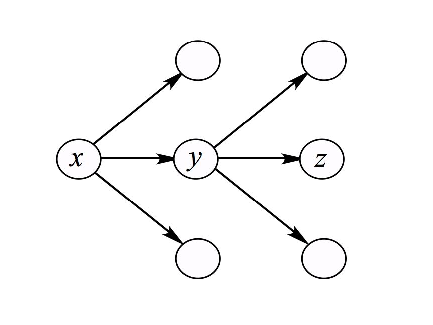
\includegraphics[width=120pt]{figure2aa}
\caption{A sample figure.}
\end{figure}

\begin{table}[h]
\caption{This is a table. }
\begin{threeparttable}
\begin{tabular}{lccrr}
\headrow
\thead{Variables} & \thead{JKL ($\boldsymbol{n=30}$)} & \thead{Control ($\boldsymbol{n=40}$)} & \thead{MN} & \thead{$\boldsymbol t$ (68)}\\
Age at testing & 38 & 58 & 504.48 & 58 ms\\
Age at testing & 38 & 58 & 504.48 & 58 ms\\
Age at testing & 38 & 58 & 504.48 & 58 ms\\
Age at testing & 38 & 58 & 504.48 & 58 ms\\
\hiderowcolors
stop alternating row colors from here onwards\\
Age at testing & 38 & 58 & 504.48 & 58 ms\\
Age at testing & 38 & 58 & 504.48 & 58 ms\\
\hline  % Please only put a hline at the end of the table
\end{tabular}

\begin{tablenotes}
\item JKL, just keep laughing; MN, merry noise.
\end{tablenotes}
\end{threeparttable}
\end{table}



\paragraph{Fourth Level Heading}
Here are examples of a quote

\begin{quote}
The significant problems we have cannot be solved at the same level of thinking with which we created them.
\end{quote}

\noindent and an epigraph

\begin{epigraph}{Albert Einstein}
Anyone who has never made a mistake has never tried anything new.
\end{epigraph}


\section*{\normalsize{ACKNOWLEDGMENTS}}
Acknowledgments should include contributions from anyone who does not meet the criteria for authorship (for example, to recognize contributions from people who provided technical help, collation of data, writing assistance, acquisition of funding, or a department chairperson who provided general support), as well as any funding or other support information.

%REFERENCES
%Note that references are placed in lexicographic order by author name. Multiple entries within a citation should appear in numerical order also, such as [2, 17, 19, 42].

%\bibliographystyle{plain}
\bibliography{sample}

\end{document} 
